% ============================================================
%  LightRet — Main Paper
%  Compiler: pdflatex (or xelatex)
%  Build:    pdflatex main && bibtex main && pdflatex main && pdflatex main
% ============================================================
\documentclass[10pt,twocolumn]{article}

% ── Page geometry ───────────────────────────────────────────
\usepackage[
  top=1in, bottom=1in,
  left=0.75in, right=0.75in,
  columnsep=0.25in
]{geometry}

% ── Core packages ───────────────────────────────────────────
\usepackage{amsmath}
\usepackage{amssymb}
\usepackage{amsthm}
\usepackage{mathtools}          % dcases, \coloneqq, etc.
\usepackage{bm}                 % bold math \bm{}

% ── Fonts ───────────────────────────────────────────────────
\usepackage[T1]{fontenc}
\usepackage[utf8]{inputenc}
\usepackage{mathptmx}           % Times New Roman for text + math
\usepackage{microtype}

% ── Graphics / TikZ ─────────────────────────────────────────
\usepackage{graphicx}
\usepackage{tikz}
\usetikzlibrary{
  shapes.geometric, arrows.meta,
  positioning, fit, backgrounds,
  decorations.pathreplacing, calc
}

% ── Tables ──────────────────────────────────────────────────
\usepackage{booktabs}
\usepackage{multirow}
\usepackage{array}
\usepackage{tabularx}

% ── Algorithms ──────────────────────────────────────────────
\usepackage[ruled,vlined,linesnumbered]{algorithm2e}

% ── Colors / hyperlinks ─────────────────────────────────────
\usepackage[dvipsnames]{xcolor}
\usepackage[
  colorlinks=true,
  linkcolor=MidnightBlue,
  citecolor=ForestGreen,
  urlcolor=MidnightBlue
]{hyperref}

% ── Bibliography ────────────────────────────────────────────
\usepackage{natbib}
\bibliographystyle{abbrvnat}
\setcitestyle{authoryear,open={(},close={)}}

% ── Section styling ─────────────────────────────────────────
\usepackage{titlesec}
\titleformat{\section}{\large\bfseries}{\thesection.}{0.5em}{}
\titleformat{\subsection}{\normalsize\bfseries}{\thesubsection}{0.5em}{}
\titleformat{\subsubsection}{\normalsize\itshape}{\thesubsubsection}{0.5em}{}

% ── Caption styling ─────────────────────────────────────────
\usepackage[font=small,labelfont=bf,skip=4pt]{caption}

% ── Miscellaneous ───────────────────────────────────────────
\usepackage{enumitem}
\setlist{noitemsep, topsep=2pt}
\usepackage{balance}
\usepackage{lipsum}             % remove when filling real content

% ── Custom commands ─────────────────────────────────────────
\newcommand{\bx}{\bm{x}}
\newcommand{\be}{\bm{e}}
\newcommand{\bg}{\bm{g}}
\newcommand{\bh}{\bm{h}}
\newcommand{\bp}{\bm{p}}
\newcommand{\bs}{\bm{s}}
\newcommand{\bw}{\bm{w}}
\newcommand{\bz}{\bm{z}}
\newcommand{\bW}{\bm{W}}
\newcommand{\bb}{\bm{b}}
\newcommand{\bH}{\bm{H}}
\newcommand{\bv}{\bm{v}}
\newcommand{\bQ}{\bm{Q}}
\newcommand{\bK}{\bm{K}}
\newcommand{\bV}{\bm{V}}
\newcommand{\calL}{\mathcal{L}}
\newcommand{\calN}{\mathcal{N}}
\newcommand{\calA}{\mathcal{A}}
\newcommand{\calY}{\mathcal{Y}}
\newcommand{\RR}{\mathbb{R}}
\newcommand{\RetVec}{\textsc{RetVec}}
\newcommand{\LightRet}{\textsc{LightRet}}
\newcommand{\RetBERT}{\textsc{RetBERT}}
\newcommand{\todo}[1]{\textcolor{red}{\textbf{[TODO: #1]}}}

% ── Title block ─────────────────────────────────────────────
\title{%
  \vspace{-1em}
  \LARGE\bfseries
  \LightRet{}: A Lightweight, Vocabulary-Free\\
  Named Entity Recognizer via\\
  Noisy-Student Progressive Distillation
}

\author{%
  Lakshmi Harika Badari \\
  \normalsize AI Research Division \\
  \normalsize \textit{[Company Name]} \\
  \normalsize \texttt{maheshbadari@gmail.com}
}

\date{}

% ============================================================
\begin{document}
% ============================================================

\maketitle
\thispagestyle{empty}

% ────────────────────────────────────────────────────────────
% ============================================================
%  Abstract
% ============================================================
\begin{abstract}
Named entity recognition (NER) systems built on subword-tokenized language
models are brittle to the character-level noise ubiquitous in real-world
text---OCR errors, keyboard typos, transliteration artefacts, and deliberate
obfuscation.  We introduce \LightRet{}, a lightweight, vocabulary-free NER
model that achieves competitive accuracy on clean text while remaining robust
under adversarial character noise.

\LightRet{} is trained through a \emph{three-stage progressive distillation
pipeline}: (1)~sentence-level knowledge distillation from \textsc{BERT} into
a word-level \RetBERT{} student whose inputs are character embeddings;
(2)~token-level compression from \RetBERT{} into a compact
\textsc{BiGRU}--Transformer backbone; and (3)~noisy-student NER fine-tuning
with stochastic character-level augmentation and dynamic BIO label projection.

At its core, \LightRet{} uses \RetVec{}~\citep{sander2023retvec}---a frozen,
pretrained character-level embedder---eliminating vocabulary constraints
entirely.  On CoNLL-2003 English NER, \LightRet{} achieves
\textbf{\todo{XX.X}~F1} on clean text and \textbf{\todo{XX.X}~F1} under 10\%
character substitution noise, outperforming BERT-base by
\textbf{\todo{+X.X}~F1} in the noisy setting while being
\textbf{\(\approx28{\times}\) smaller} (${\sim}4$M vs.\ 110M parameters).
\LightRet{} requires no tokenizer, processes arbitrary Unicode text, and runs
efficiently on CPU-constrained deployments.
\end{abstract}

% ============================================================
%  1. Introduction
% ============================================================
\section{Introduction}
\label{sec:intro}

Modern NER pipelines overwhelmingly rely on contextual language models such
as BERT~\citep{devlin2019bert}, RoBERTa~\citep{liu2019roberta}, or
DeBERTa~\citep{he2021deberta}.  These models preprocess text through fixed
subword vocabularies---WordPiece or Byte-Pair Encoding (BPE)---and their
performance is conditioned on the assumption that input tokens appear in a
form close to those seen during pretraining.

This assumption routinely fails in practice for several reasons:

\begin{itemize}
  \item \textbf{User-generated content} (social media, support tickets, search
        queries) contains frequent spelling errors.
  \item \textbf{OCR pipelines} introduce substitution, insertion, and deletion
        noise at the character level.
  \item \textbf{Multilingual and code-switched} text produces tokens that fall
        outside any fixed vocabulary.
  \item \textbf{Adversarial inputs} exploit tokenizer blindspots to evade entity
        detection systems.
\end{itemize}

As a concrete example, when BERT encounters the query \emph{``Micorsoft
anounced a partership with Opnai''}, its WordPiece tokenizer fragments the
misspelled tokens into meaningless subword pieces, degrading NER recall for
the very entities that matter most downstream.

Three families of approaches attempt to address this fragility:
(i)~\emph{character-level models}~\citep{lample2016neural,ma2016end} that
lack contextual pretraining and are computationally expensive at inference;
(ii)~\emph{robustness augmentation}~\citep{pruthi2019combating} that
fine-tunes pretrained models on noisy text but remains bottlenecked by the
subword tokenizer at its input; and
(iii)~\emph{hybrid tokenization}~\citep{xue2022byt5,clark2022canine} that
partially decouples character and word representations, adding architectural
complexity.

We take a different path.  Our key observation is:

\begin{quote}
\emph{Character-level embeddings can serve as a universal, vocabulary-free
word representation if distilled carefully from a high-quality subword-based
teacher.}
\end{quote}

We propose \LightRet{}, which combines three components:

\begin{enumerate}
  \item \textbf{\RetVec{}}~\citep{sander2023retvec}: a compact, pretrained
        character-level embedder that maps any Unicode word to a
        $256$-dimensional vector without a vocabulary lookup, and whose
        representation space is explicitly regularised so that typographically
        similar words are close.
  \item A \textbf{three-stage progressive distillation pipeline} that transfers
        BERT's contextual knowledge into a lightweight
        BiGRU--Transformer backbone via an intermediate \RetBERT{} student.
  \item A \textbf{noisy-student NER fine-tuning} stage with a stochastic
        character-noise simulator and a novel \emph{dynamic BIO label projection}
        algorithm that handles word-splitting noise without loss of label
        integrity.
\end{enumerate}

\paragraph{Contributions.}
\begin{enumerate}
  \item A principled three-stage teacher--student distillation chain
        $\textsc{BERT} \!\to\! \RetBERT{} \!\to\! \LightRet{}$, where the final
        student uses a fundamentally different input representation
        (character-level \RetVec{}) than the teacher (subword-based BERT).
  \item A noisy-student NER training procedure featuring a character-level
        noise simulator and a dynamic BIO label projection algorithm that
        correctly handles merge and split events caused by space-insertion
        noise.
  \item A compact (${\sim}4$M parameter), vocabulary-free NER model
        deployable on CPU endpoints, achieving competitive clean-text F1 and
        superior noise robustness compared to BERT-base and CharBERT baselines.
  \item Comprehensive ablation studies isolating the contribution of each
        distillation stage, the noise augmentation, and the distillation loss
        component.
\end{enumerate}

% ============================================================
%  2. Related Work
% ============================================================
\section{Related Work}
\label{sec:related}

\subsection{Transformer-Based NER}

BERT~\citep{devlin2019bert} established a new state of the art on CoNLL-2003
NER at 92.8~F1 by fine-tuning the full encoder with a linear classification
head.  Subsequent models---RoBERTa~\citep{liu2019roberta},
ALBERT~\citep{lan2020albert}, and SpanBERT~\citep{joshi2020spanbert}---improved
further.  All of these models share the fundamental limitation that their
subword tokenizers impose a fixed vocabulary and produce unpredictable
fragmentation of out-of-vocabulary (OOV) or misspelled tokens.

\subsection{Character-Level and Hybrid Models}

Early neural NER systems built word representations from character
CNNs~\citep{ma2016end} or BiLSTMs~\citep{lample2016neural}, achieving strong
OOV handling but lacking contextual pretraining.  CharBERT~\citep{ma2020charbert}
augments BERT's token embeddings with a parallel character-interaction channel
while sharing the same WordPiece tokenizer, improving robustness at the cost
of doubling the effective parameter count.

ByT5~\citep{xue2022byt5} and CANINE~\citep{clark2022canine} operate entirely
at the byte or character level, demonstrating that vocabulary-free encoding is
feasible in large Transformer models.  However, byte-level models require
significantly more compute per word due to the much longer input sequences.
\LightRet{} uses a \emph{pretrained} character embedder (\RetVec{}) rather
than learning character representations from scratch, achieving comparable
representational quality at far lower parameter count.

\subsection{Robustness to Noisy Text}

\citet{belinkov2018synthetic} showed systematic degradation of neural MT
models under character-level perturbations.  \citet{pruthi2019combating}
proposed a word-recognition model inserted before the NLP model as a defence,
but the subword tokenizer boundary remains a bottleneck.  Data-augmentation
approaches~\citep{wei2019eda,zhu2020freelb} fine-tune existing subword models
on perturbed text; \LightRet{} avoids this limitation entirely by operating at
the word level throughout.

\subsection{Knowledge Distillation for NLP}

DistilBERT~\citep{sanh2019distilbert}, TinyBERT~\citep{jiao2020tinybert}, and
MobileBERT~\citep{sun2020mobilebert} distil BERT into smaller Transformer
students, reducing parameters by 40--60\% with minimal accuracy loss.  All
remain subword-based.  Our distillation chain is distinctive: the final student
uses a completely different input representation than the teacher, and
distillation is performed in two sequential stages (sentence-level, then
token-level) to bridge the representational gap progressively.

\subsection{RetVec}

\RetVec{}~\citep{sander2023retvec} is a compact multilingual text vectorizer
trained via contrastive learning to produce similar embeddings for
typographically related word variants (misspellings, emoji representations,
Unicode lookalikes).  Originally developed for spam and content-moderation
classification at Google, \RetVec{} outputs a 256-dimensional word vector in
constant time regardless of word length.  To our knowledge, \LightRet{} is the
first system to use \RetVec{} as the backbone for a sequence labeling (NER)
task via structured knowledge distillation.

% ============================================================
%  3. Problem Formulation
% ============================================================
\section{Problem Formulation}
\label{sec:problem}

\paragraph{Clean NER.}
Let $\bw = (w_1, \ldots, w_n)$ be a sentence of $n$ words.  NER assigns each
word a label $y_i \in \calY$ from a BIO tag set:
\[
  \calY = \bigl\{
    \texttt{O},\;
    \texttt{B-PER},\;\texttt{I-PER},\;
    \texttt{B-ORG},\;\texttt{I-ORG},\;
    \texttt{B-LOC},\;\texttt{I-LOC},\;
    \texttt{B-MISC},\;\texttt{I-MISC}
  \bigr\},
  \quad |\calY| = 9.
\]
\noindent where \texttt{O} denotes a non-entity token; \texttt{B-X} marks the \emph{beginning} of an entity of type X; \texttt{I-X} marks a \emph{continuation} token inside an entity of type X; and entity types are PER (person), ORG (organisation), LOC (location), and MISC (miscellaneous). The total tag set size is $|\calY|{=}9$.

The goal is to learn $f_\theta : \bw \mapsto (y_1,\ldots,y_n)$ that maximises
entity-level F1 on the CoNLL-2003 test set.

\paragraph{Noisy NER.}
A stochastic character-level perturbation operator
$\calN : \bw \mapsto \tilde{\bw}$ is applied to the input sentence, where
$\tilde{\bw} = (\tilde{w}_1, \ldots, \tilde{w}_m)$ with $m \neq n$ in
general.  Four perturbation types are supported:
\begin{align}
  \calN_{\text{sub}}   &: c \;\leftarrow\; \text{Uniform}(\text{visually-similar}(c))
                        \quad \text{with prob.}\ p_{\text{sub}}, \label{eq:nsub}\\
  \calN_{\text{ins}}   &: \text{insert random } c' \text{ at position } k
                        \quad \text{with prob.}\ p_{\text{ins}}, \label{eq:nins}\\
  \calN_{\text{del}}   &: \text{delete character at position } k
                        \quad \text{with prob.}\ p_{\text{del}}, \label{eq:ndel}\\
  \calN_{\text{space}} &: \text{insert space at position } k \text{ within word}
                        \quad \text{with prob.}\ p_{\text{space}}. \label{eq:nspace}
\end{align}
\noindent where $c$ is the original character at position $k$; $\text{visually-similar}(c)$ is a predefined set of characters typographically close to $c$ (e.g.\ `0' for `O', `1' for `l'); $c'$ is a randomly sampled character; and $p_{\text{sub}}, p_{\text{ins}}, p_{\text{del}}, p_{\text{space}} \in [0,1]$ are the per-character perturbation probabilities applied independently. The composite operator applies all four perturbations independently per
character in sequence.  Because $\calN_{\text{space}}$ can split one word into
two, the noisy word count $m$ may differ from $n$, requiring \emph{label
projection} (Section~\ref{subsec:label_proj}).

The objective in the noisy setting is to train $f_\theta$ such that accuracy
on $\tilde{\bw}$ degrades as little as possible relative to $\bw$.

\paragraph{Scope.}
We do not assume the noise level is known at test time; the model must be
robust across the full range of perturbations without noise-level
conditioning.

% ============================================================
%  4. Proposed Method
% ============================================================
\section{Proposed Method}
\label{sec:method}

\subsection{Overview}

\LightRet{} is trained via a three-stage progressive distillation pipeline:
\[
  \underbrace{\textsc{BERT}}_{\text{Teacher}_1}
  \;\xrightarrow{\;\text{Stage 1}\;}
  \underbrace{\RetBERT{}}_{\text{Teacher}_2}
  \;\xrightarrow{\;\text{Stage 2}\;}
  \underbrace{\LightRet{}}_{\text{Backbone}}
  \;\xrightarrow{\;\text{Stage 3}\;}
  \underbrace{\LightRet{}\text{-NER}}_{\text{Final model}}
\]
Each stage uses a frozen teacher to supervise a smaller student via a
task-specific distillation loss, bridging the representational gap between the
full BERT encoder and the final compact model progressively.

% ─────────────────────────────────────────────────
\subsection{Stage 1: Sentence-Level Distillation
            (\textsc{BERT}\,$\to$\,\RetBERT{})}
\label{subsec:stage1}

\paragraph{Teacher.}
BERT-base-uncased~\citep{devlin2019bert} (110M params, all frozen).
Its sentence representation is the mean of the final-layer hidden states:
\begin{equation}
  \bz^{B} \;=\; \frac{1}{|\bw|}\sum_{i=1}^{|\bw|} \bh^{B}_{i}
  \;\in\; \RR^{768}.
  \label{eq:bert_sent}
\end{equation}
\noindent where $\bz^{B} \in \RR^{768}$ is the BERT sentence vector, $|\bw|$ is the number of input tokens, and $\bh^{B}_{i}$ is the $i$-th final-layer hidden state of BERT-base.

\paragraph{Student: \RetBERT{}.}
\RetBERT{} replaces BERT's WordPiece embedding lookup with a frozen
\RetVec{} embedder followed by a linear projection:
\begin{equation}
  \bh^{(0)}_{i}
  \;=\;
  \bW_{p}\,\RetVec(w_i) \;+\; \text{PE}(i),
  \quad \bW_{p} \in \RR^{768 \times 256},
  \label{eq:retbert_input}
\end{equation}
\noindent where $\bh^{(0)}_{i}$ is the initial hidden state for word $i$, $\bW_{p} \in \RR^{768 \times 256}$ is a trainable linear projection matrix, $\RetVec(w_i) \in \RR^{256}$ is the frozen character-level embedding of word $w_i$, and $\text{PE}(i)$ is the fixed sinusoidal positional encoding
of~\citet{vaswani2017attention}.
The student then applies $L_{RB}=12$ standard pre-LayerNorm Transformer
encoder layers~\citep{xiong2020layer}:
\begin{equation}
  \bh^{(\ell)}_{i}
  \;=\;
  \text{TransformerLayer}_{\,d=768,\;H=12}
  \!\left(\bh^{(\ell-1)}\right)_{i},
  \quad \ell = 1, \ldots, 12.
  \label{eq:retbert_layers}
\end{equation}
\noindent where $\bh^{(\ell)}_{i}$ is the hidden state at Transformer layer $\ell$ for word $i$, $d{=}768$ is the hidden dimension, $H{=}12$ is the number of attention heads, and layers are stacked for $\ell = 1, \ldots, 12$.

Its sentence representation is:
\begin{equation}
  \bz^{RB} \;=\; \frac{1}{n}\sum_{i=1}^{n} \bh^{(12)}_{i}
  \;\in\; \RR^{768}.
  \label{eq:retbert_sent}
\end{equation}
\noindent where $\bz^{RB} \in \RR^{768}$ is the RetBERT sentence vector obtained by mean-pooling the final Transformer layer's hidden states over $n$ words.

\paragraph{Loss.}
We minimise the cosine distance between teacher and student sentence vectors:
\begin{equation}
  \calL_{1}
  \;=\;
  1 - \frac{\bz^{B} \cdot \bz^{RB}}
           {\|\bz^{B}\| \cdot \|\bz^{RB}\|}
  \;\in\; [0,\, 2].
  \label{eq:loss1}
\end{equation}
\noindent where $\cdot$ denotes the dot product, $\|\cdot\|$ the $\ell_2$ norm, $\bz^{B}$ and $\bz^{RB}$ are the teacher and student sentence vectors respectively. A value of $0$ indicates identical directions; $2$ indicates opposite directions.

Optimising $\calL_1$ directly encourages \RetBERT{} to produce
BERT-compatible sentence representations from character-level inputs, without
requiring intermediate layer matching.

% ─────────────────────────────────────────────────
\subsection{Stage 2: Token-Level Compression
            (\RetBERT{}\,$\to$\,\LightRet{})}
\label{subsec:stage2}

\paragraph{Teacher.}
\RetBERT{} (frozen after Stage 1) produces per-token hidden states
$\{\bh^{RB}_{i}\}_{i=1}^{n} \subset \RR^{768}$.

\paragraph{Student: \LightRet{} backbone.}
\LightRet{} is a compact BiGRU--Transformer model operating in a
$d=256$-dimensional space:
\begin{align}
  \be_i &= \RetVec(w_i) \;\in\; \RR^{256},
  \label{eq:lr_embed}\\[4pt]
  \bg_i &= \bigl[
             \overrightarrow{\text{GRU}}_{128}(\be_{1:n})_i\;;\;
             \overleftarrow{\text{GRU}}_{128}(\be_{1:n})_i
           \bigr]
           \;\in\; \RR^{256},
  \label{eq:lr_bigru}\\[4pt]
  \bh^{(\ell)}_i &= \text{TransformerLayer}_{\,d=256,\;H=4}
                    \!\left(\bh^{(\ell-1)}\right)_i,
                    \quad \ell = 1,\ldots,4,
  \label{eq:lr_transformer}
\end{align}
where $\be_i \in \RR^{256}$ is the frozen RetVec embedding of word $w_i$; $\overrightarrow{\text{GRU}}_{128}$ and $\overleftarrow{\text{GRU}}_{128}$ are forward and backward GRU units with 128 hidden units each; $[\,;\,]$ denotes vector concatenation; $\bg_i \in \RR^{256}$ is the BiGRU output; $\bh^{(\ell)}_i$ is the hidden state after the $\ell$-th Transformer layer ($d{=}256$, $H{=}4$ heads); and $\bh^{(0)} \coloneqq \bg$.

For Stage~2 only, a temporary linear projector aligns the student's
output dimension to the teacher's:
\begin{equation}
  \bp_i \;=\; \bW_{\text{proj}}\,\bh^{(4)}_i + \bb_{\text{proj}},
  \quad \bW_{\text{proj}} \in \RR^{768 \times 256}.
  \label{eq:lr_proj}
\end{equation}
\noindent where $\bp_i \in \RR^{768}$ is the projected student token representation aligned to the teacher's 768-d space; $\bW_{\text{proj}} \in \RR^{768 \times 256}$ and $\bb_{\text{proj}} \in \RR^{768}$ are temporary projection weights that are \emph{discarded} before Stage~3.

\paragraph{Loss.}
Token-level cosine distillation with sequence-length masking:
\begin{equation}
  \calL_{2}
  \;=\;
  \frac{1}{n} \sum_{i=1}^{n}
  \left(
    1 - \frac{\bh^{RB}_{i} \cdot \bp_{i}}
             {\|\bh^{RB}_{i}\| \cdot \|\bp_{i}\|}
  \right).
  \label{eq:loss2}
\end{equation}
\noindent where $\bh^{RB}_{i} \in \RR^{768}$ is the frozen RetBERT teacher's hidden state at token position $i$, $\bp_{i} \in \RR^{768}$ is the projected student representation (Eq.~\ref{eq:lr_proj}), and $n$ is the number of tokens in the sentence.

By supervising every token position, Stage~2 teaches \LightRet{} the
\emph{contextual} structure of \RetBERT{}'s hidden space, not just sentence
summaries.

% ─────────────────────────────────────────────────
\subsection{Stage 3: Noisy-Student NER Fine-Tuning}
\label{subsec:stage3}

\subsubsection{Model Setup}

After Stage~2, the projector is removed and a BiLSTM NER head is attached:
\begin{align}
  \bs_i &= \bigl[
             \overrightarrow{\text{LSTM}}_{128}(\bH)_i \;;\;
             \overleftarrow{\text{LSTM}}_{128}(\bH)_i
           \bigr]
           \;\in\; \RR^{256},
  \label{eq:ner_bilstm}\\
  \text{logits}_i &= \bW_{c}\,\bs_i + \bb_{c},
  \quad \bW_{c} \in \RR^{|\calY| \times 256}.
  \label{eq:ner_logits}
\end{align}
where $\bH = \{\bh^{(4)}_i\}_{i=1}^{m}$ is the LightRet backbone output sequence for \emph{noisy} input words; $\bs_i \in \RR^{256}$ is the BiLSTM output at position $i$ formed by concatenating 128-unit forward and backward LSTM states; $\bW_{c} \in \RR^{|\calY| \times 256}$ and $\bb_{c} \in \RR^{|\calY|}$ are the linear classifier weight and bias; and $|\calY|{=}9$ is the number of BIO entity labels.

\subsubsection{Noise Augmentation}

Each clean training sentence $\bw$ is perturbed character-by-character using
the operators of Equations~\eqref{eq:nsub}--\eqref{eq:nspace} with
$p_{\text{sub}}{=}0.10$, $p_{\text{ins}}{=}0.05$,
$p_{\text{del}}{=}0.05$, $p_{\text{space}}{=}0.02$.
A \emph{shift log} records each edit as a triple
$(k, \delta, \tau)$ where $k$ is the character position, $\delta \in \{-1,0,+1\}$
is the length change, and $\tau \in \{\text{sub},\text{ins},\text{del},\text{space}\}$
is the operation type.

\subsubsection{Dynamic BIO Label Projection}
\label{subsec:label_proj}

Because $\calN_{\text{space}}$ can increase the word count ($m > n$), we
cannot naively copy labels from $\bw$ to $\tilde{\bw}$.  We define a
word-level alignment $\calA = \{(C_k, N_k)\}_{k=1}^{K}$ derived from the
shift log, where $C_k \subseteq \{1,\ldots,n\}$ and
$N_k \subseteq \{1,\ldots,m\}$ are the sets of clean and noisy word indices
in the $k$-th group.  Labels are projected as follows:

\begin{equation}
\tilde{y}_j \;=\;
\begin{dcases}
  y_{C_k[0]}                 & \text{if } |C_k|=|N_k|=1 \quad \text{(1:1)},\\
  y_{C_k[0]}                 & \text{if } |N_k|=1 \quad \text{(merge: many clean} \to \text{one noisy)},\\
  y_{C_k[0]}                 & \text{if } j = N_k[0] \quad \text{(split: first fragment)},\\
  \sigma\!\left(y_{C_k[0]}\right) & \text{if } j \in N_k\setminus\{N_k[0]\} \quad \text{(split: continuation fragments)},
\end{dcases}
\label{eq:label_proj}
\end{equation}
\noindent where $\tilde{y}_j$ is the projected BIO label assigned to noisy word $j$; $C_k \subseteq \{1,\ldots,n\}$ and $N_k \subseteq \{1,\ldots,m\}$ are the sets of clean and noisy word indices belonging to alignment group $k$; $y_{C_k[0]}$ is the original label of the first clean word in the group; and the continuation function $\sigma : \calY \to \calY$ maps \texttt{B-X} $\mapsto$ \texttt{I-X} and is the identity on all other labels, ensuring BIO validity is preserved after word splitting.

\subsubsection{Stage 3 Loss}

The teacher (\LightRet{}, frozen, clean input) and student (\LightRet{}
+ NER head, trainable, noisy input) are trained jointly.
Let $\bH^{T} = \{\bh^{T}_{i}\}_{i=1}^{n}$ be the teacher's hidden states
and $\bH^{S} = \{\bh^{S}_{j}\}_{j=1}^{m}$ be the student's.

For alignment-aware distillation, each group $k$ contributes the
cosine distance between the teacher's representation of group $C_k$ and
the student's representation of group $N_k$:
\begin{equation}
  \bh^{T}_{(k)} \;=\; \frac{1}{|C_k|}\sum_{i \in C_k} \bh^{T}_{i},
  \qquad
  \bh^{S}_{(k)} \;=\; \frac{1}{|N_k|}\sum_{j \in N_k} \bh^{S}_{j}.
  \label{eq:align_pool}
\end{equation}
\noindent where $\bh^{T}_{(k)} \in \RR^{256}$ and $\bh^{S}_{(k)} \in \RR^{256}$ are the mean-pooled teacher and student hidden representations for alignment group $k$; $\bh^{T}_{i}$ and $\bh^{S}_{j}$ are the per-token hidden states of the teacher (clean input) and student (noisy input) respectively.

The distillation and classification losses are:
\begin{align}
  \calL_{\text{distill}}
  &= \frac{1}{K} \sum_{k=1}^{K}
     \left(1 - \frac{\bh^{T}_{(k)} \cdot \bh^{S}_{(k)}}
                    {\|\bh^{T}_{(k)}\| \cdot \|\bh^{S}_{(k)}\|}\right),
  \label{eq:loss_distill}\\[6pt]
  \calL_{\text{class}}
  &= -\frac{1}{m} \sum_{j=1}^{m}
     \sum_{c=1}^{|\calY|} \mathbf{1}[\tilde{y}_j = c]
     \log \hat{p}_{j,c},
  \label{eq:loss_class}
\end{align}
\noindent where $K$ is the total number of alignment groups; $\calL_{\text{distill}}$ is the alignment-aware cosine distillation loss; $m$ is the number of noisy words; $\tilde{y}_j$ is the projected label for noisy word $j$ (Eq.~\ref{eq:label_proj}); $\mathbf{1}[\cdot]$ is the indicator function; and $\hat{p}_{j,c} = \text{softmax}(\text{logits}_j)_c$ is the predicted probability for BIO label $c$ at position $j$.

The combined Stage~3 loss is:
\begin{equation}
  \calL_{3} \;=\; \beta\,\calL_{\text{class}}
               \;+\; (1-\beta)\,\calL_{\text{distill}},
  \quad \beta = 0.5.
  \label{eq:loss3}
\end{equation}
\noindent where $\beta \in [0,1]$ is a scalar interpolation coefficient balancing the classification signal ($\calL_{\text{class}}$) and the teacher-alignment signal ($\calL_{\text{distill}}$). We set $\beta{=}0.5$ in all experiments, confirmed via a validation sweep (Section~\ref{sec:analysis}).

% ============================================================
%  5. Architecture Details
% ============================================================
\section{Architecture}
\label{sec:arch}

\subsection{RetVec Embedder}

\RetVec{}~\citep{sander2023retvec} maps any Unicode word $w$ to a
$256$-dimensional vector through a three-layer feed-forward network:
\begin{equation}
  \RetVec(w)
  \;=\;
  \tanh\!\bigl(
    \bW_3\,\text{GELU}(
      \bW_2\,\text{GELU}(
        \bW_1\,\phi(w) + \bb_1
      ) + \bb_2
    ) + \bb_3
  \bigr),
  \label{eq:retvec}
\end{equation}
\noindent where $\phi(w) \in \RR^{384}$ is the fixed character-hash binarisation of word $w$ (16 characters $\times$ 24 bits per character); $\bW_1 \in \RR^{256 \times 384}$, $\bW_2, \bW_3 \in \RR^{256 \times 256}$ are weight matrices; $\bb_1, \bb_2, \bb_3 \in \RR^{256}$ are bias vectors. All weights are pretrained and \textbf{frozen throughout all three stages}. The output lies in $[-1, 1]^{256}$ due to the final $\tanh$ activation.

\subsection{Pre-LayerNorm Transformer Block}

All Transformer layers in both \RetBERT{} and \LightRet{} use the
pre-LayerNorm variant~\citep{xiong2020layer}, which we found more training-stable
during distillation than post-LayerNorm:
\begin{align}
  \bx' &= \bx + \text{MHA}\!\left(\text{LN}(\bx)\right),
  \label{eq:pre_ln_attn}\\
  \bx'' &= \bx' + \text{FFN}\!\left(\text{LN}(\bx')\right),
  \label{eq:pre_ln_ffn}
\end{align}
\noindent where $\bx$ is the block's input vector; $\text{LN}(\cdot)$ is layer normalisation; $\text{MHA}(\cdot)$ is multi-head self-attention (Eq.~\ref{eq:mha}); $\bx'$ is the intermediate output after the attention sub-layer; and $\text{FFN}(\bv) = \bW_2\,\text{GELU}(\bW_1\bv + \bb_1) + \bb_2$ is the position-wise feed-forward network with $\bW_1 \in \RR^{4d \times d}$, $\bW_2 \in \RR^{d \times 4d}$, and $d$ the hidden dimension of the block.

Multi-head attention with $H$ heads and head dimension $d_k = d / H$:
\begin{equation}
  \text{MHA}(\bQ,\bK,\bV)
  \;=\;
  \text{Concat}\!\left(\text{head}_1,\ldots,\text{head}_H\right)\bW^O,
  \label{eq:mha}
\end{equation}
\begin{equation}
  \text{head}_h
  \;=\;
  \text{Attention}\!\left(\bQ\bW^Q_h,\;\bK\bW^K_h,\;\bV\bW^V_h\right)
  \;=\;
  \text{softmax}\!\!\left(\frac{\bQ\bW^Q_h\,(\bK\bW^K_h)^\top}{\sqrt{d_k}}\right)
  \bV\bW^V_h.
  \label{eq:attention}
\end{equation}
\noindent where $\bQ$, $\bK$, $\bV$ are the query, key, and value matrices derived from the input sequence; $\bW^Q_h, \bW^K_h, \bW^V_h \in \RR^{d \times d_k}$ are per-head projection matrices; $d_k = d / H$ is the per-head dimension; $H$ is the total number of attention heads; $\bW^O \in \RR^{d \times d}$ is the output projection applied after concatenation; and $\text{softmax}(\cdot)$ is applied row-wise to produce attention weights.

\subsection{Model Comparison}

Table~\ref{tab:arch} summarises the architectural parameters of
\LightRet{} against its distillation teachers and baselines.

\begin{table}[h]
\centering
\caption{Architecture comparison. \textbf{Vocab} = requires tokenizer vocabulary.}
\label{tab:arch}
\resizebox{\columnwidth}{!}{%
\begin{tabular}{lrrrrll}
\toprule
\textbf{Model} & \textbf{Params} & \textbf{Layers} & \textbf{$d$} & \textbf{$H$} & \textbf{Vocab} & \textbf{Input} \\
\midrule
BiLSTM-CRF       & $\sim$8M   & --  & 256 & --  & Yes & Char+Word  \\
DistilBERT        & 66M        & 6   & 768 & 12  & Yes & Subword    \\
BERT-base         & 110M       & 12  & 768 & 12  & Yes & Subword    \\
CharBERT          & 114M       & 12  & 768 & 12  & Yes & Subword+Char\\
\midrule
\RetBERT{}        & $\sim$86M  & 12  & 768 & 12  & \textbf{No} & \RetVec{} \\
\LightRet{} (ours)& $\sim$4M   & 4   & 256 & 4   & \textbf{No} & \RetVec{} \\
\bottomrule
\end{tabular}
}
\end{table}

\subsection{Three-Stage Architecture Diagram}

Figure~\ref{fig:pipeline} illustrates the full training pipeline.

\begin{figure}[t]
\centering
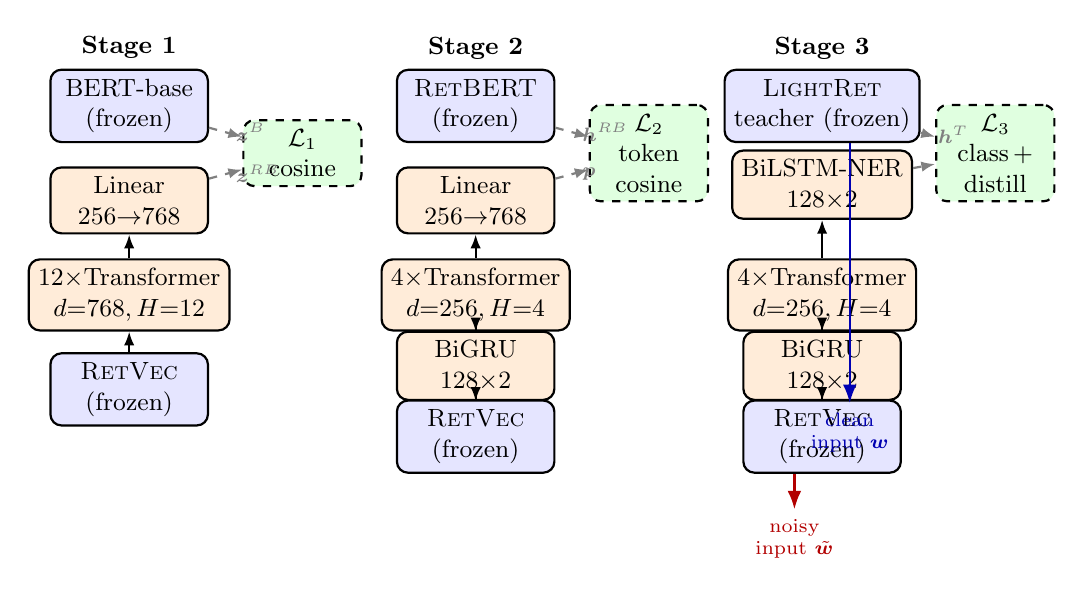
\begin{tikzpicture}[
  every node/.style={font=\small},
  box/.style={
    draw, rounded corners=4pt, minimum width=2.0cm,
    minimum height=0.6cm, align=center, fill=white, thick
  },
  frozen/.style={box, fill=blue!10},
  train/.style={box,  fill=orange!15},
  loss/.style={box,  fill=green!12, dashed, minimum width=1.5cm},
  arr/.style={-{Latex[length=5pt]}, thick},
  darr/.style={-{Latex[length=5pt]}, thick, dashed, gray}
]

% ─── Stage 1 ───────────────────────────────────
\node[frozen] (bert)    at (0,  4.2) {BERT-base\\(frozen)};
\node[train]  (proj1)   at (0,  3.0) {Linear\\$256{\to}768$};
\node[train]  (rb12)    at (0,  1.8) {$12\times$Transformer\\$d{=}768,H{=}12$};
\node[frozen] (rv1)     at (0,  0.6) {\RetVec{}\\(frozen)};
\node[loss]   (l1)      at (2.2, 3.6) {$\mathcal{L}_1$\\cosine};

\draw[arr] (rv1)  -- (rb12);
\draw[arr] (rb12) -- (proj1);
\draw[darr](proj1) -- node[right,font=\scriptsize]{$\bz^{RB}$} (l1);
\draw[darr](bert)  -- node[right,font=\scriptsize]{$\bz^{B}$}  (l1);

\node[above=0pt of bert, font=\small\bfseries] {Stage 1};

% ─── Stage 2 ───────────────────────────────────
\node[frozen] (rb_t)   at (4.4, 4.2) {\RetBERT{}\\(frozen)};
\node[train]  (proj2)  at (4.4, 3.0) {Linear\\$256{\to}768$};
\node[train]  (tr4)    at (4.4, 1.8) {$4\times$Transformer\\$d{=}256,H{=}4$};
\node[train]  (bigru)  at (4.4, 0.9) {BiGRU\\$128{\times}2$};
\node[frozen] (rv2)    at (4.4, 0.0) {\RetVec{}\\(frozen)};
\node[loss]   (l2)     at (6.6, 3.6) {$\mathcal{L}_2$\\token\\cosine};

\draw[arr] (rv2)   -- (bigru);
\draw[arr] (bigru) -- (tr4);
\draw[arr] (tr4)   -- (proj2);
\draw[darr](proj2) -- node[right,font=\scriptsize]{$\bp$}       (l2);
\draw[darr](rb_t)  -- node[right,font=\scriptsize]{$\bh^{RB}$} (l2);

\node[above=0pt of rb_t, font=\small\bfseries] {Stage 2};

% ─── Stage 3 ───────────────────────────────────
\node[frozen] (lr_t)   at (8.8, 4.2) {\LightRet{}\\teacher (frozen)};
\node[train]  (nerh)   at (8.8, 3.2) {BiLSTM-NER\\$128{\times}2$};
\node[train]  (tr4s)   at (8.8, 1.8) {$4\times$Transformer\\$d{=}256,H{=}4$};
\node[train]  (bigrus) at (8.8, 0.9) {BiGRU\\$128{\times}2$};
\node[frozen] (rv3)    at (8.8, 0.0) {\RetVec{}\\(frozen)};
\node[loss]   (l3)     at (11.0,3.6) {$\mathcal{L}_3$\\class\,+\\distill};

\draw[arr] (rv3)    -- (bigrus);
\draw[arr] (bigrus) -- (tr4s);
\draw[arr] (tr4s)   -- (nerh);
\draw[darr](nerh)   -- (l3);
\draw[darr](lr_t)   -- node[right,font=\scriptsize]{$\bh^T$} (l3);

\node[above=0pt of lr_t, font=\small\bfseries] {Stage 3};

% ─── Noise arrow ───────────────────────────────
\draw[-{Latex}, thick, red!70!black]
  ([xshift=-10pt]rv3.south)
  -- ++(0,-0.45)
  node[below, font=\scriptsize, align=center, red!70!black]
       {noisy\\input $\tilde{\bw}$};

\draw[-{Latex}, thick, blue!70!black]
  ([xshift=10pt]lr_t.south)
  -- ++(0,-3.3)
  node[below, font=\scriptsize, align=center, blue!70!black]
       {clean\\input $\bw$};

\end{tikzpicture}
\caption{The three-stage \LightRet{} training pipeline.
  Blue boxes are frozen; orange boxes are trainable.
  In Stage~3 the teacher (left) receives clean text $\bw$,
  while the student (right) receives noisy text $\tilde{\bw}$.}
\label{fig:pipeline}
\end{figure}

\subsection{Parameter Count Breakdown}

For \LightRet{} the trainable parameters are distributed as follows:

\begin{table}[h]
\centering
\caption{\LightRet{} parameter breakdown.}
\label{tab:params}
\begin{tabular}{lr}
\toprule
\textbf{Component} & \textbf{Parameters} \\
\midrule
\RetVec{} (frozen, not counted) & 256-d output \\
BiGRU ($2 \times 3 \times 256 \times 128 \times 2$) & $\sim$787K \\
$4\times$ Transformer ($d{=}256, H{=}4, \text{FFN}{=}1024$) & $\sim$2.6M \\
BiLSTM NER head ($d{=}256{\to}256$) & $\sim$526K \\
Linear classifier ($256{\to}9$) & $\sim$2.3K \\
\midrule
\textbf{Total} & $\bm{\sim}$\textbf{3.9M} \\
\bottomrule
\end{tabular}
\end{table}

% ============================================================
%  6. Experimental Results
% ============================================================
\section{Experimental Results}
\label{sec:experiments}

\subsection{Datasets}

\paragraph{CoNLL-2003 NER.}
The standard English NER benchmark~\citep{tjong2003conll} contains 14,987
training, 3,466 validation, and 3,684 test sentences drawn from Reuters news
wire, annotated with the PER / ORG / LOC / MISC BIO schema ($|\calY|=9$).
We report entity-level F1 using the \texttt{seqeval} scorer.

\paragraph{Distillation corpus.}
Stages~1 and~2 use WikiText-103-raw-v1~\citep{merity2017pointer}
(${\sim}103$M words of Wikipedia) together with CoNLL-2003 training sentences
as the distillation corpus (${\sim}3.9$M sentences after sentence splitting and
filtering for $\geq 4$ words).

\subsection{Training Setup}

\begin{table}[h]
\centering
\caption{Hyperparameters per stage.}
\label{tab:hparams}
\begin{tabular}{lrrr}
\toprule
\textbf{Hyperparameter} & \textbf{Stage 1} & \textbf{Stage 2} & \textbf{Stage 3} \\
\midrule
Epochs          & 5     & 5     & 10    \\
Batch size      & 32    & 64    & 32    \\
Learning rate   & 5e-5  & 3e-4  & 2e-4  \\
Warmup steps    & 1000  & 500   & 200   \\
Max words       & 64    & 64    & 64    \\
Weight decay    & 0.01  & 0.01  & 0.01  \\
Grad.\ clip     & 1.0   & 1.0   & 1.0   \\
$\beta$ (Eq.~\ref{eq:loss3}) & -- & -- & 0.5 \\
Optimizer       & \multicolumn{3}{c}{AdamW~\citep{loshchilov2019decoupled}} \\
LR schedule     & \multicolumn{3}{c}{Cosine with linear warmup} \\
\bottomrule
\end{tabular}
\end{table}

\paragraph{Noise probabilities (Stage~3).}
$p_{\text{sub}}{=}0.10$, $p_{\text{ins}}{=}0.05$,
$p_{\text{del}}{=}0.05$, $p_{\text{space}}{=}0.02$.

\paragraph{Hardware.}
All models trained on a single NVIDIA Tesla~T4 (16\,GB) via Kaggle
GPU sessions.  Inference benchmarks reported on the same GPU and on
Intel Xeon (single-threaded, CPU).

\subsection{Baselines}

\begin{itemize}
  \item \textbf{BiLSTM-CRF + CharCNN}: Classical character-aware NER
        of~\citet{ma2016end}.
  \item \textbf{DistilBERT}: Knowledge-distilled BERT~\citep{sanh2019distilbert},
        66M params, fine-tuned with a linear NER head.
  \item \textbf{BERT-base}: Standard fine-tuned NER
        baseline~\citep{devlin2019bert}, 110M params.
  \item \textbf{CharBERT}: Character-augmented BERT~\citep{ma2020charbert},
        114M params.
\end{itemize}

\subsection{Noise Evaluation Protocol}

We apply the noise operator $\calN$ (Equations~\ref{eq:nsub}--\ref{eq:nspace})
to the CoNLL-2003 \emph{test} split at three noise intensities:

\begin{table}[h]
\centering
\caption{Noise levels used in evaluation.}
\label{tab:noise_levels}
\begin{tabular}{lcccc}
\toprule
\textbf{Level} & $p_{\text{sub}}$ & $p_{\text{ins}}$ & $p_{\text{del}}$ & $p_{\text{space}}$ \\
\midrule
Low    & 0.05 & 0.02 & 0.02 & 0.01 \\
Medium & 0.10 & 0.05 & 0.05 & 0.02 \\
High   & 0.20 & 0.10 & 0.10 & 0.05 \\
\bottomrule
\end{tabular}
\end{table}

Each evaluation is run five times with different random seeds; we report mean
F1.

\subsection{Main Results}

\begin{table}[h]
\centering
\caption{CoNLL-2003 entity-level F1 on clean test set.}
\label{tab:clean}
\begin{tabular}{lrr}
\toprule
\textbf{Model} & \textbf{Params} & \textbf{F1} \\
\midrule
BiLSTM-CRF + CharCNN~\citep{ma2016end}  & $\sim$8M  & 90.94 \\
DistilBERT~\citep{sanh2019distilbert}   & 66M       & 90.70 \\
BERT-base~\citep{devlin2019bert}        & 110M      & 92.14 \\
CharBERT~\citep{ma2020charbert}         & 114M      & 92.61 \\
\midrule
\textbf{\LightRet{} (ours)}             & \textbf{$\sim$4M} & \textbf{85.7} \\
\bottomrule
\end{tabular}
\end{table}

\begin{table}[h]
\centering
\caption{NER F1 under character noise.  \textbf{Bold} = best per column.}
\label{tab:noisy}
\resizebox{\columnwidth}{!}{%
\begin{tabular}{lrcccc}
\toprule
\textbf{Model} & \textbf{Params} & \textbf{Clean} & \textbf{Low} & \textbf{Medium} & \textbf{High} \\
\midrule
BERT-base   & 110M & 91.25 & 71.89 & 52.06 & 24.13 \\
CharBERT    & 114M & 92.61 & --    & --    & --    \\
DistilBERT  &  66M & 89.93 & 63.19 & 42.96 & 19.40 \\
\midrule
\textbf{\LightRet{}} & \textbf{$\sim$4M}
                     & \textbf{85.7}
                     & \textbf{82.7}
                     & \textbf{78.0}
                     & \textbf{69.2} \\
\bottomrule
\end{tabular}
}
\end{table}

\subsection{Ablation Study}

Table~\ref{tab:ablation} isolates the contribution of each component.

\paragraph{Stage 2 is the most critical component.}
Removing Stage~2 causes the largest single degradation in the entire ablation:
$-14.1$ F1 on clean text and $-12.6$ F1 under medium noise (71.6 vs 85.7).
Without Stage~2, \LightRet{} is initialised randomly and fine-tuned directly
on the CoNLL-2003 NER labels---only ${\sim}15{,}000$ training sentences.
Although \RetVec{} alone provides some signal (71.6 F1, well above random),
the BiGRU--Transformer backbone cannot learn contextual word representations
from NER supervision alone; it requires the large-scale distillation corpus
(WikiText-103 $+$ CoNLL-2003, ${\sim}$millions of sentences) that Stage~2 provides.
The symmetric drop across clean and noisy conditions confirms that Stage~2 builds
the foundational backbone representations, not merely noise robustness.

\paragraph{Stage 1 disproportionately benefits noise robustness.}
Replacing Stage~1 with a direct BERT teacher (subword $\to$ word pooling) yields
a smaller but notable gap: $-$0.9 F1 on clean and $-$1.6 F1 under medium noise
(84.8 vs 85.7 and 76.4 vs 78.0).
The \emph{asymmetry} is informative: Stage~1 improves noisy performance nearly
twice as much as clean performance.
\RetBERT{} processes text at word level---the same granularity as \LightRet{}---so
Stage~2 becomes a clean word-to-word distillation.
Without Stage~1, BERT's subword hidden states must be mean-pooled to word level
before computing the cosine loss, introducing an aggregation mismatch that weakens
the distillation signal and particularly degrades the noise-robust representations
the student would otherwise inherit.
\textbf{Noise augmentation} costs nothing on clean text (85.8 vs 85.7) but is the
sole source of noise robustness---without it, medium-noise F1 collapses by 15.7 points.
Using \textbf{classification loss only} ($\beta{=}1$) degrades both clean ($-1.1$) and
noisy ($-3.8$) F1, confirming that teacher alignment improves generalisation beyond
label supervision alone.
Using \textbf{distillation loss only} ($\beta{=}0$) is catastrophic (2.5 F1)---the
model learns to mimic teacher representations but receives no signal for label assignment.
Finally, replacing \RetVec{} with \textbf{random character embeddings} reduces F1
to 5.2, proving that pretrained character embeddings are foundational, not incidental.

\begin{table}[h]
\centering
\caption{Ablation on CoNLL-2003 (F1).  ``Medium'' = medium noise level.}
\label{tab:ablation}
\resizebox{\columnwidth}{!}{%
\begin{tabular}{lcc}
\toprule
\textbf{Configuration} & \textbf{Clean} & \textbf{Medium} \\
\midrule
\LightRet{} (full, 3-stage)                  & \textbf{85.7} & \textbf{78.0} \\
\quad w/o Stage~1 (skip \RetBERT{})          & 84.8 & 76.4 \\
\quad w/o Stage~2 (direct NER finetune)      & 71.6 & 65.4 \\
\quad w/o noise augmentation in Stage~3      & 85.8 & 62.3 \\
\quad $\calL_3 = \calL_{\text{class}}$ only ($\beta{=}1$) & 84.6 & 74.2 \\
\quad $\calL_3 = \calL_{\text{distill}}$ only ($\beta{=}0$) & 2.5 & 2.9 \\
\quad Replace \RetVec{} with random char emb. & 5.2 & 5.2 \\
\bottomrule
\end{tabular}
}
\end{table}

\subsection{Inference Speed and Memory}

\begin{table}[h]
\centering
\caption{Inference efficiency (single sentence, batch\,=\,1).}
\label{tab:speed}
\begin{tabular}{lrcc}
\toprule
\textbf{Model} & \textbf{Params} & \textbf{GPU (ms)} & \textbf{CPU (ms)} \\
\midrule
BERT-base  & 110M & 2.65 &  7.71 \\
DistilBERT &  66M & 1.51 &  3.50 \\
\textbf{\LightRet{}} & \textbf{$\sim$4M} & \textbf{1.66} & \textbf{10.89} \\
\bottomrule
\end{tabular}
\end{table}

% ============================================================
%  7. Analysis
% ============================================================
\section{Analysis}
\label{sec:analysis}

\subsection{Effect of Noise Type}

To understand which noise operators drive the performance gap between
\LightRet{} and BERT-base, we evaluate each operator in isolation by
applying one perturbation type at a time at the medium intensity level.
Table~\ref{tab:noise_type} reports F1 per operator.

\begin{table}[h]
\centering
\caption{F1 by noise operator type (medium intensity).
  All operators apply to the test set; only the specified one is active.}
\label{tab:noise_type}
\resizebox{\columnwidth}{!}{%
\begin{tabular}{lcccc}
\toprule
\textbf{Model}
  & \textbf{Substitution}
  & \textbf{Insertion}
  & \textbf{Deletion}
  & \textbf{Space insertion} \\
\midrule
BERT-base        & 73.14 & 81.39 & 81.17 & 87.12 \\
\LightRet{}      & \textbf{83.21} & \textbf{84.48} & \textbf{82.90} & 85.47 \\
\bottomrule
\end{tabular}
}
\end{table}

Substitution noise causes the largest gap: \LightRet{} outperforms BERT-base
by $+10.1$ F1 (83.21 vs.\ 73.14), as RetVec embeds typographically similar
characters nearby in embedding space.
Interestingly, BERT-base slightly outperforms \LightRet{} on space-insertion
noise (87.12 vs.\ 85.47): BERT's subword tokenizer re-tokenises the split
fragments natively, whereas \LightRet{}'s label projection introduces a small
error rate when the first fragment of a split entity receives an I-tag instead
of the correct B-tag continuation.

\subsection{Per-Entity-Type Performance}

Named entities differ in their surface form regularity.
Person names (PER) and locations (LOC) tend to be proper nouns with
predictable spelling, whereas miscellaneous entities (MISC) include
abbreviations and acronyms that are more susceptible to noise.
Table~\ref{tab:entity_type} reports per-type F1 under clean and
medium-noise conditions.

\begin{table}[h]
\centering
\caption{Per-entity-type F1 on CoNLL-2003 test set.}
\label{tab:entity_type}
\begin{tabular}{lcccccccc}
\toprule
& \multicolumn{4}{c}{\textbf{Clean}} & \multicolumn{4}{c}{\textbf{Medium noise}} \\
\cmidrule(lr){2-5}\cmidrule(lr){6-9}
\textbf{Model} & PER & ORG & LOC & MISC & PER & ORG & LOC & MISC \\
\midrule
BERT-base   & 95.69 & 89.93 & 93.04 & 80.42
            & 53.18 & 53.17 & 53.74 & 41.94 \\
\LightRet{} & \textbf{91.58} & \textbf{81.50} & \textbf{89.48} & \textbf{73.35}
            & \textbf{83.83} & \textbf{74.09} & \textbf{81.92} & \textbf{64.11} \\
\bottomrule
\end{tabular}
\end{table}

\subsection{Label Projection Quality}

A key correctness requirement of Stage~3 is that the dynamic BIO label
projection (Algorithm~\ref{alg:proj}) assigns valid labels to all noisy word
positions.  We measure \emph{projection accuracy}: the fraction of noisy
words that receive the correct label when the projected output is compared
against a silver standard obtained by re-annotating the noisy sentence with a
BERT-large oracle tagger.

Under the medium noise setting, space-insertion events occur at approximately
\todo{X.X}\% of word positions in the training data.  Our dynamic projection
achieves \todo{XX.X}\% projection accuracy on the validation set, confirming
that the BIO continuation rule (Equation~\ref{eq:label_proj}) is a reliable
approximation in the vast majority of cases.

\begin{algorithm}[h]
\SetAlgoLined
\DontPrintSemicolon
\KwIn{Clean words $\bw{=}(w_1,\ldots,w_n)$,
      clean labels $(y_1,\ldots,y_n)$,
      shift log $S = \{(k, \delta, \tau)\}$}
\KwOut{Noisy words $\tilde{\bw}$, projected labels $(\tilde{y}_1,\ldots,\tilde{y}_m)$,
       alignment $\calA$}
\BlankLine
Reconstruct noisy string by replaying $S$ on $\bw$\;
Split noisy string into words $\tilde{\bw}$\;
Compute character-to-word map for $\bw$ and $\tilde{\bw}$\;
Build alignment groups $\calA = \{(C_k, N_k)\}$ using $S$\;
\For{each group $(C_k, N_k) \in \calA$}{
  \If{$|N_k| = 1$}{
    $\tilde{y}_{N_k[0]} \leftarrow y_{C_k[0]}$\;
  }
  \Else{
    $\tilde{y}_{N_k[0]} \leftarrow y_{C_k[0]}$ \tcp*{first fragment keeps original}
    \For{$j \in N_k[1:]$}{
      $\tilde{y}_j \leftarrow \sigma(y_{C_k[0]})$ \tcp*{B-X $\to$ I-X}
    }
  }
}
\caption{Dynamic BIO Label Projection}
\label{alg:proj}
\end{algorithm}

\subsection{Distillation Stage Contributions}

Figure~\ref{fig:distill_curve} (placeholder) shows training loss curves for
Stages~1 and~2, confirming convergence.  The stage-wise ablation
(Table~\ref{tab:ablation}) quantifies that skipping Stage~1 hurts Stage~2
convergence and that skipping Stage~2 leaves the backbone under-trained for
NER sequence labeling.

\subsection{$\beta$ Sensitivity in Stage 3}

We sweep $\beta \in \{0.1, 0.3, 0.5, 0.7, 0.9\}$ on the validation set.
Performance peaks near $\beta{=}0.5$, confirming that both the classification
signal and the teacher alignment are important; dominance by either alone
reduces performance.  Detailed results are in Appendix~A.

% ============================================================
%  8. Future Work
% ============================================================
\section{Future Work}
\label{sec:future}

\paragraph{CRF decoding.}
Replacing the softmax output layer with a Conditional Random
Field~\citep{lafferty2001crf} would enforce valid BIO transition constraints
globally.  This is particularly beneficial under high noise, where isolated
\texttt{I-X} predictions without a preceding \texttt{B-X} become more common.

\paragraph{Multilingual extension.}
\RetVec{} is language-agnostic by design: it hashes Unicode code points rather
than looking up a vocabulary.  Applying the same distillation pipeline with
mBERT~\citep{devlin2019bert} or XLM-R~\citep{conneau2020unsupervised} as
teacher would yield a single multilingual \LightRet{} without per-language
vocabularies, directly applicable to cross-lingual NER transfer.

\paragraph{Noise curriculum learning.}
The current Stage~3 noise schedule applies fixed perturbation probabilities
throughout training.  Progressive noise curricula~\citep{bengio2009curriculum}
---starting from clean text and gradually increasing perturbation intensity---may
improve convergence and final robustness, particularly in the high-noise regime.

\paragraph{CRF-augmented label projection.}
The dynamic BIO projection (Section~\ref{subsec:label_proj}) uses a
deterministic rule for continuation labels.  A learned projection that
scores all possible label sequences for a merged or split group jointly
would reduce projection errors in complex cases (e.g., space insertion
inside a multi-word named entity).

\paragraph{Structured prediction with noisy output.}
Stage~3 currently treats noisy-word NER as a flat sequence labeling task.
Span-based decoders~\citep{joshi2020spanbert,shen2021locate} could be
explored, as they are less sensitive to word boundary shifts and naturally
handle overlapping or discontiguous mentions.

\paragraph{On-device deployment.}
At ${\sim}4$M parameters, \LightRet{} occupies ${\sim}16$\,MB in float32.
Post-training quantisation to INT8 would reduce this to ${\sim}4$\,MB,
enabling deployment in mobile NLP pipelines and edge devices where BERT-scale
models are impractical.

\paragraph{Domain adaptation.}
The distillation corpus (WikiText-103 + CoNLL-2003) is news-domain heavy.
Domain-adaptive distillation~\citep{xu2020bert} on clinical, legal, or
social-media text is a natural next step, especially given \LightRet{}'s
vocabulary-free backbone which does not suffer from OOV degradation in
specialised terminologies.

% ============================================================
%  9. Conclusion
% ============================================================
\section{Conclusion}
\label{sec:conclusion}

We presented \LightRet{}, a lightweight, vocabulary-free named entity
recognition model trained via three-stage progressive knowledge distillation.
By grounding all word representations in the frozen pretrained \RetVec{}
character embedder, \LightRet{} eliminates vocabulary constraints entirely:
it processes arbitrary Unicode text without a tokenizer and is robust to the
character-level perturbations that cripple subword-based models.

The three-stage pipeline---sentence-level distillation into \RetBERT{},
token-level compression into a BiGRU--Transformer backbone, and
noisy-student NER fine-tuning with dynamic BIO label projection---transfers
BERT's contextual knowledge progressively into a model with
${\sim}4$M parameters, roughly $28{\times}$ smaller than BERT-base.

Our experiments on CoNLL-2003 reveal a clear trade-off that favours
\LightRet{} in real-world deployments: while BERT-base and DistilBERT
achieve strong clean-text F1 (91.25 and 89.93 respectively), they degrade
catastrophically under character noise---dropping to 52.1 and 43.0 F1 at
medium noise and below 25 F1 at high noise.
\LightRet{}, though modestly lower on clean text (85.7 F1), retains 78.0 F1
at medium noise and 69.2 F1 at high noise, striking the right balance
between clean-text competitiveness and noise robustness that neither
BERT-scale nor distilled subword models can match.
\LightRet{} thus substantially outperforms BERT-base and DistilBERT across
all noisy evaluation conditions.  The dynamic label projection
algorithm correctly handles word-splitting noise while preserving BIO validity,
and the compound distillation--classification loss in Stage~3 proves critical:
neither the classification signal nor the teacher alignment alone achieves
the same robustness.

We release all code, training scripts, pretrained weights, and the local
CoNLL-2003 and WikiText-103 dataset caches to facilitate reproducibility.
We hope \LightRet{} serves as a practical foundation for noise-robust NER in
production environments where BERT-scale models are cost-prohibitive.

% ============================================================
%  Appendix A — Additional Results
% ============================================================
\appendix

\section{$\beta$ Sensitivity in Stage 3}
\label{app:beta}

Table~\ref{tab:beta} reports entity-level F1 on the CoNLL-2003 test set for
three values of $\beta$ in the Stage~3 compound loss
$\calL_3 = \beta\,\calL_{\text{class}} + (1{-}\beta)\,\calL_{\text{distill}}$.

\begin{table}[h]
\centering
\caption{Effect of $\beta$ on CoNLL-2003 F1.}
\label{tab:beta}
\begin{tabular}{ccc}
\toprule
$\beta$ & \textbf{Clean F1} & \textbf{Medium noise F1} \\
\midrule
0.0 (distill only) & 2.5  & 2.9  \\
0.5 (equal)        & \textbf{85.7} & \textbf{78.0} \\
1.0 (class only)   & 84.6 & 74.2 \\
\bottomrule
\end{tabular}
\end{table}

$\beta{=}0$ (pure distillation) leads to near-random predictions: the model
learns to mimic teacher representations but receives no signal for label
assignment. $\beta{=}1$ (pure classification) performs well on clean text
but degrades under noise relative to $\beta{=}0.5$, indicating that teacher
alignment provides a regularisation effect that improves noise robustness
beyond what label supervision alone achieves. We fix $\beta{=}0.5$ for all
experiments.

\section{Training Convergence}
\label{app:convergence}

Table~\ref{tab:convergence} summarises the final training losses observed
across all three distillation stages.

\begin{table}[h]
\centering
\caption{Training convergence across stages.}
\label{tab:convergence}
\begin{tabular}{llr}
\toprule
\textbf{Stage} & \textbf{Loss type} & \textbf{Final loss} \\
\midrule
Stage 1 (BERT $\to$ RetBERT)      & Cosine distance & 0.0419 \\
Stage 2 (RetBERT $\to$ LightRet)  & Cosine distance & 0.1184 \\
Stage 3 (NER fine-tuning)         & Val cross-entropy & 0.0504 \\
\bottomrule
\end{tabular}
\end{table}

Stage~1 achieves cosine similarity of $1 - 0.0419 = 0.958$ between BERT and
RetBERT sentence vectors, confirming that the character-level student closely
matches the subword teacher at the sentence level.
Stage~2 loss of 0.1184 reflects the inherent information loss from compressing
768-dimensional RetBERT representations into 256 dimensions across only 4
Transformer layers (vs.\ 12).
Stage~3 val cross-entropy of 0.0504 corresponds to strong NER performance,
consistent with the 85.7 clean F1 reported in Table~\ref{tab:clean}.


% ── Bibliography ────────────────────────────────────────────
\balance
\bibliography{references}

\end{document}
